\chapter{Development}

\label{ch:Development}

\setlength{\parindent}{4em}
\setlength{\parskip}{1em}
\renewcommand{\baselinestretch}{1.5}

\section{Chamber for the experiment}
Because we use the light to stimulate the subject,so we need to have the light that enters the subject's retina are only from the stimulus, also help to increase an accuracy of the result. Therefore, we use the experiment chamber from our senior project.

The chamber is made from PVC pipeline and black fabric. The dimension of the chamber is W x D x H : 1.5 x 1.5 x 1.9 meters.

\begin{figure}[ht]
	\centering
	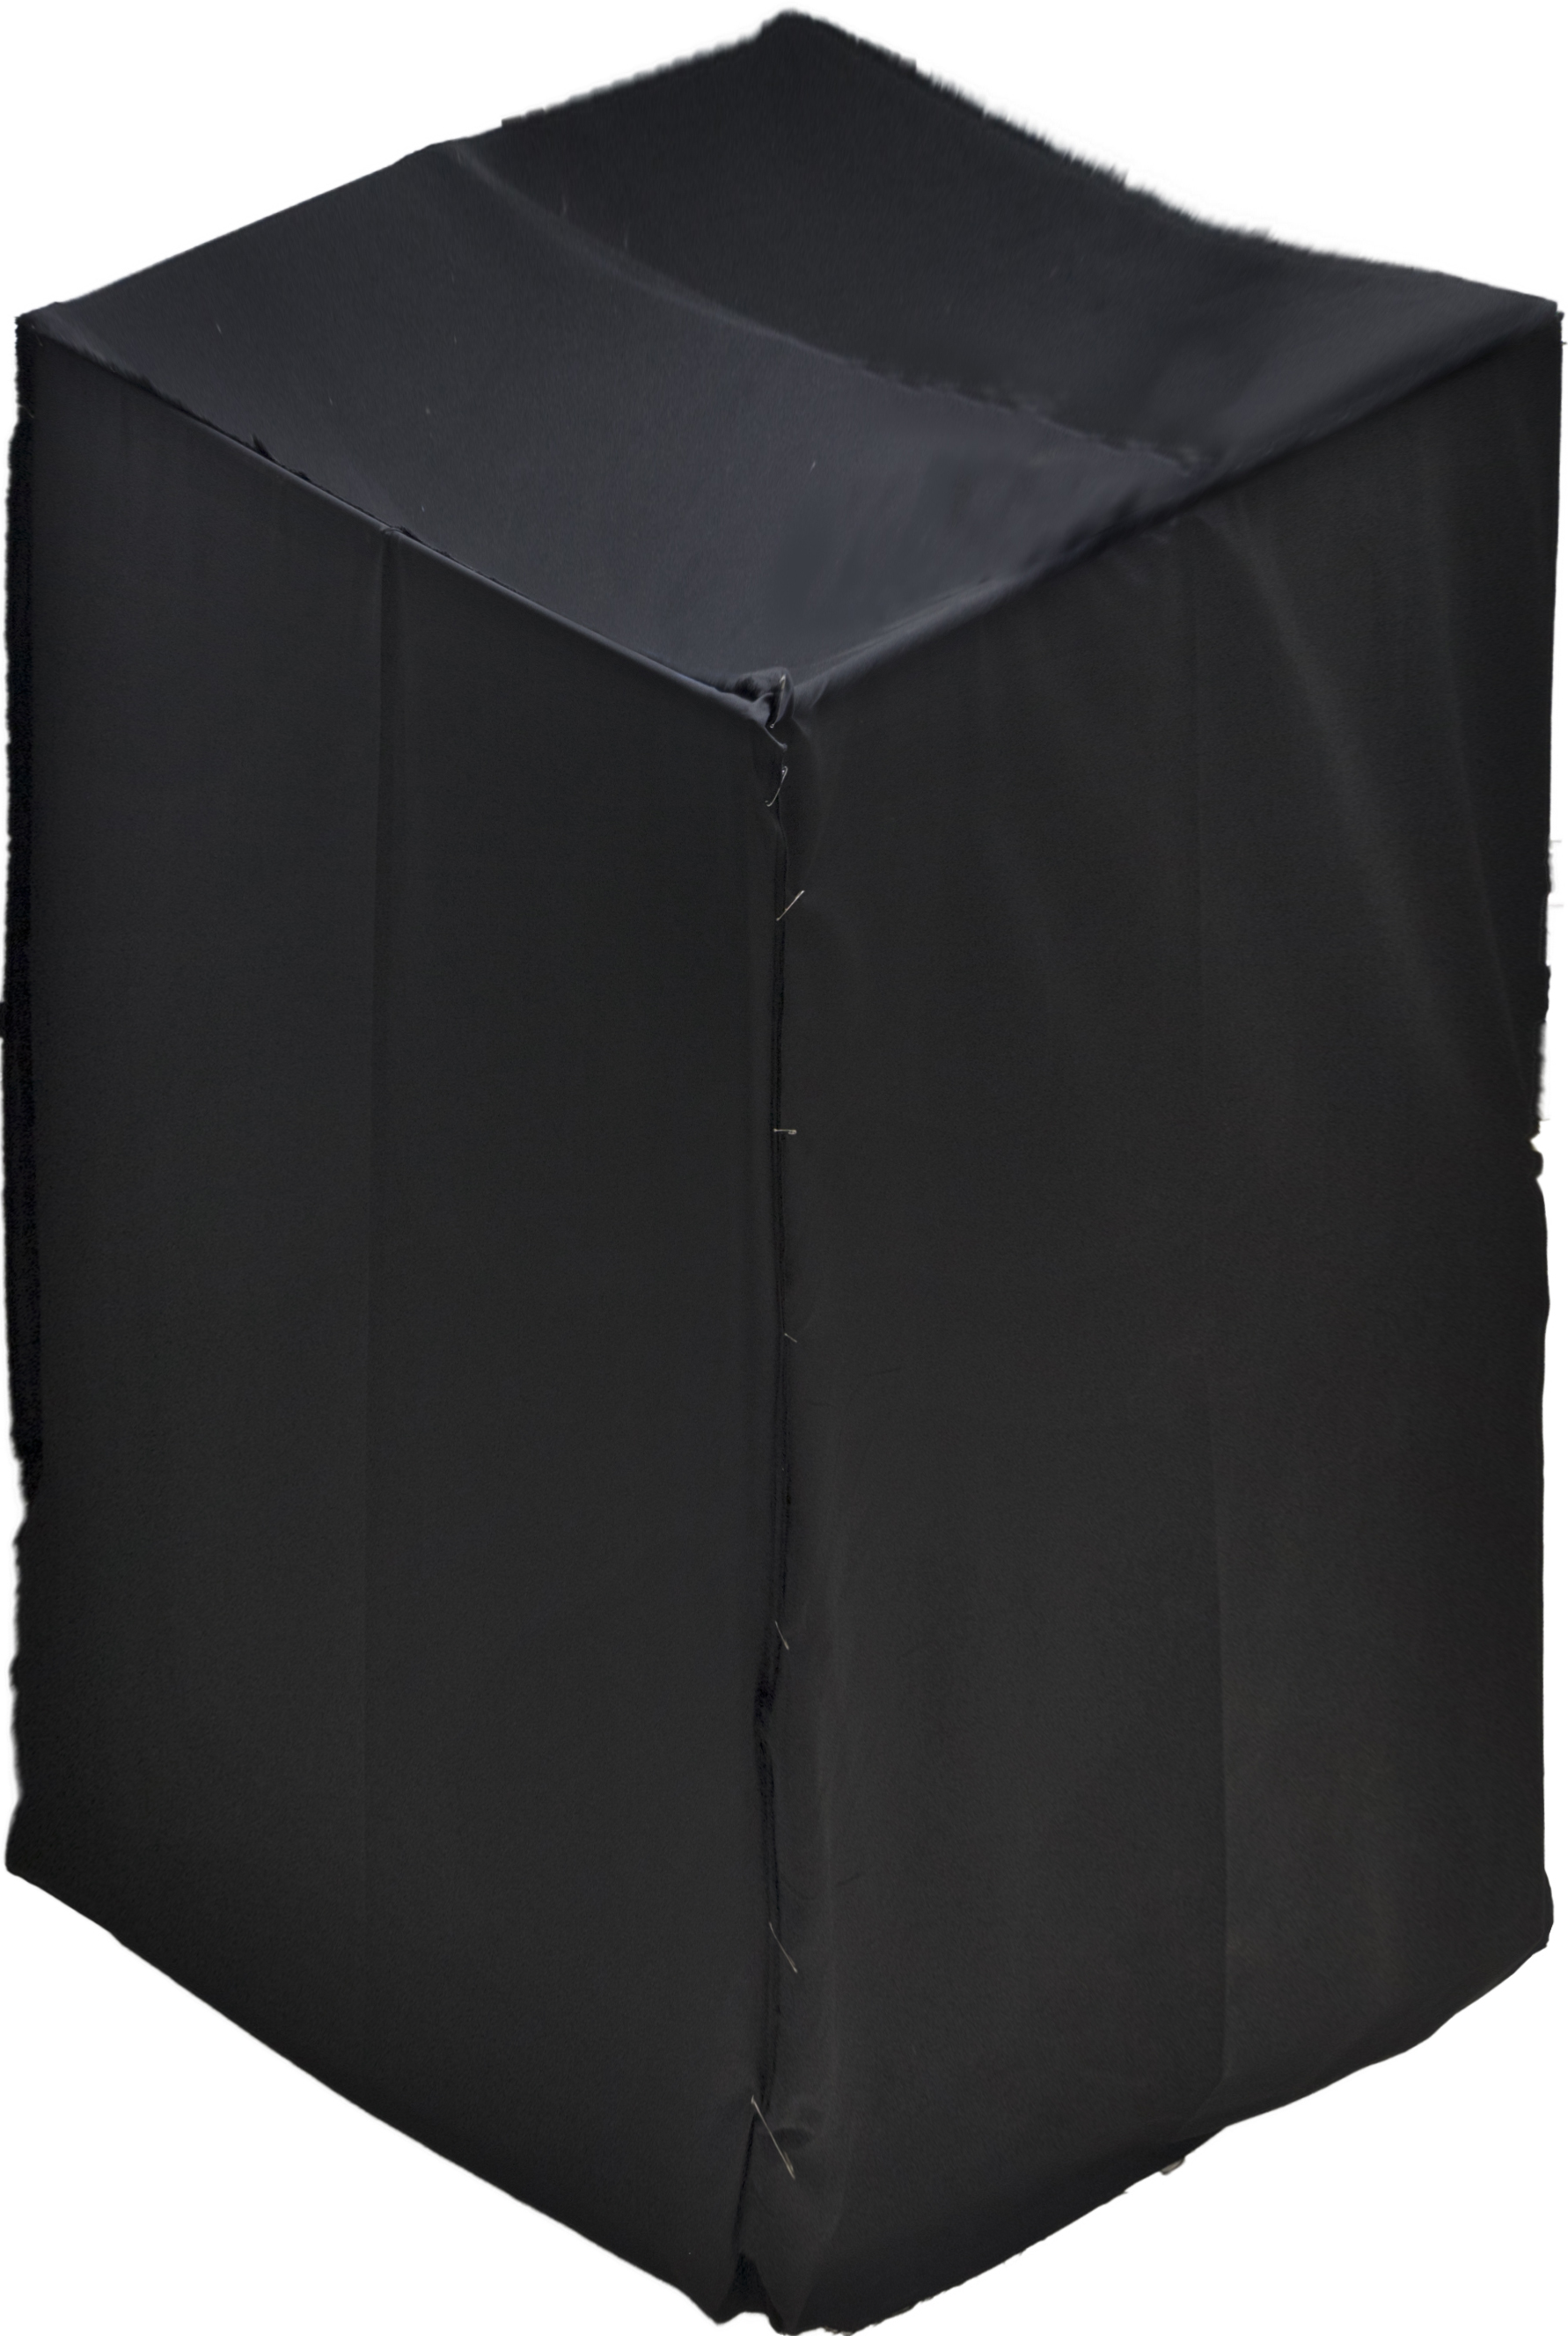
\includegraphics[width=0.4\textwidth]{chapter6/blackbox.jpg}
	\caption{Experiment Chamber}
\end{figure}

\begin{figure}[ht]
	\centering
	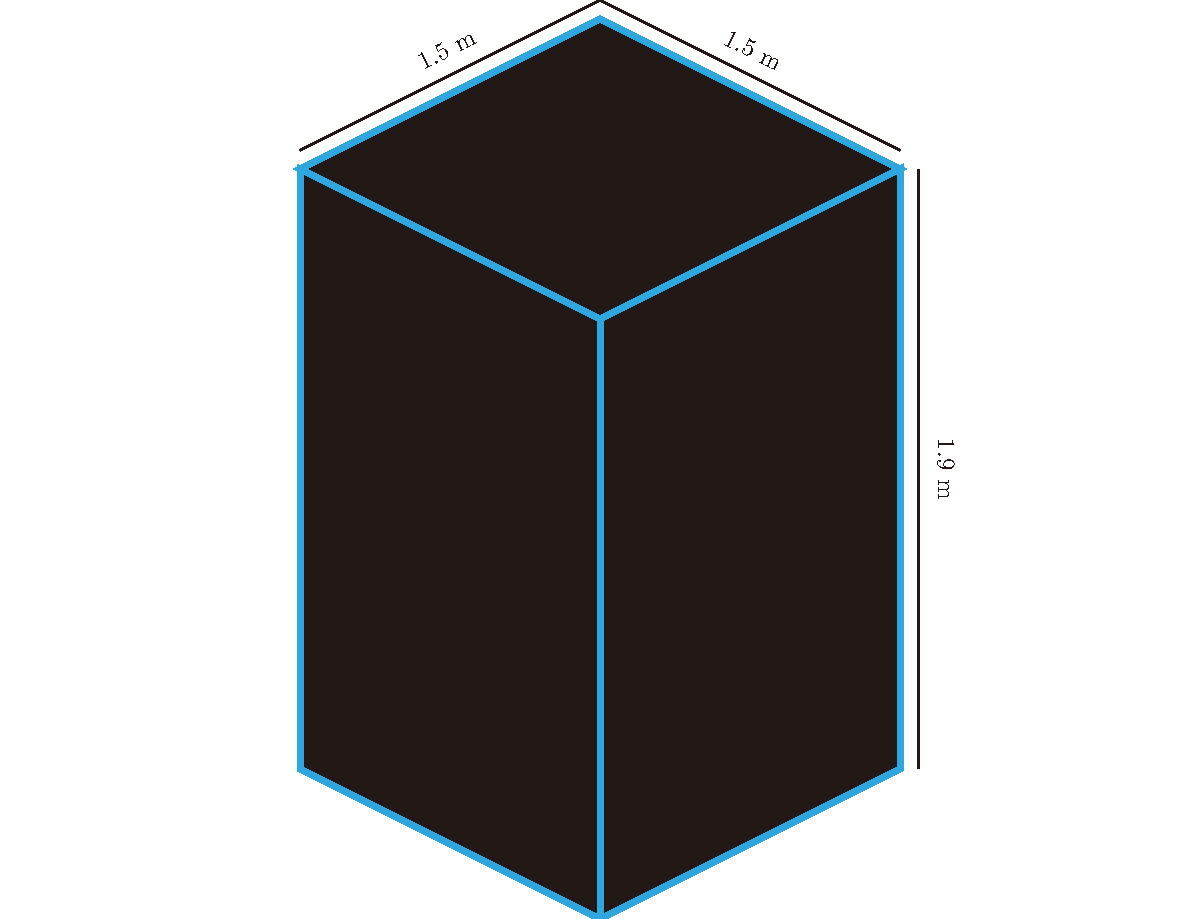
\includegraphics[width=0.8\textwidth]{chapter6/dark_wire.pdf}
	\caption{Experiment Chamber dimension}
\end{figure}

\begin{figure}[ht]
	\centering
	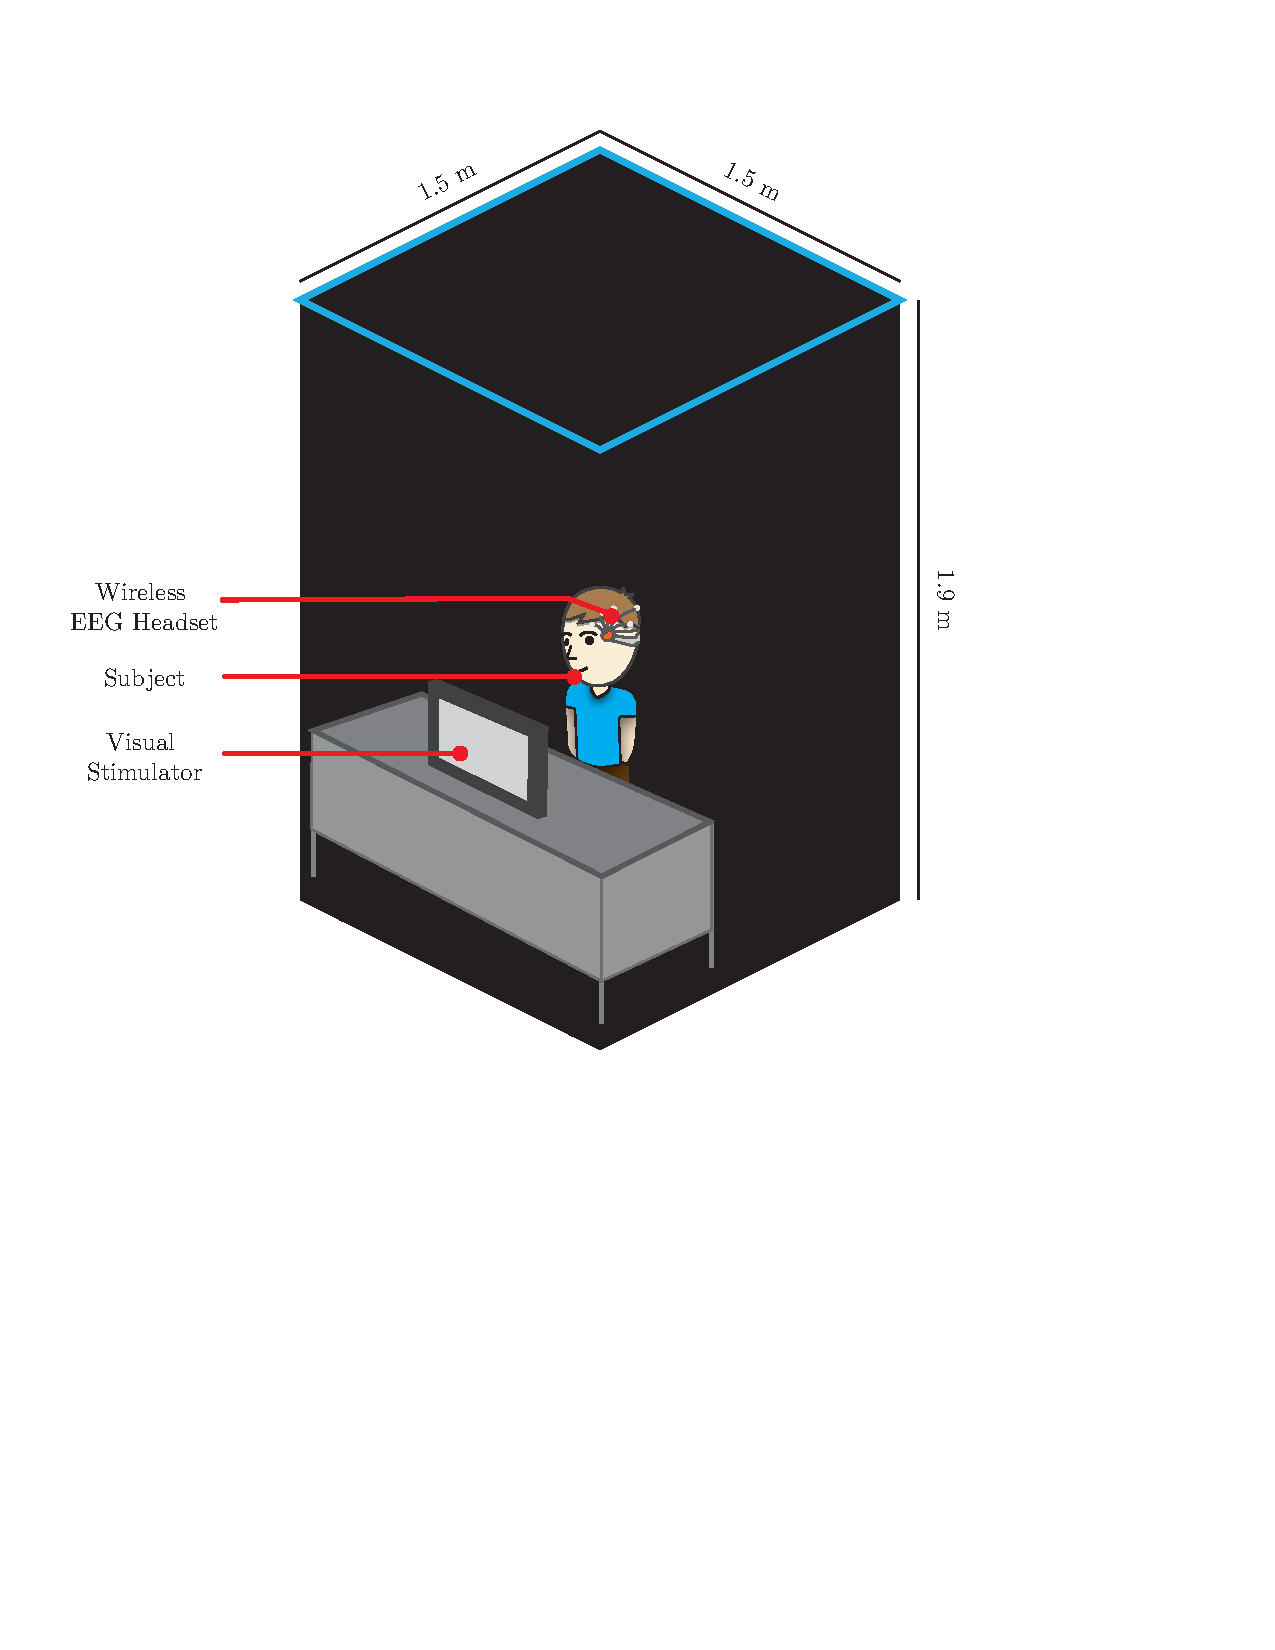
\includegraphics[width=0.8\textwidth]{chapter6/dark_wire_inside.pdf}
	\caption{Inside experiment Chamber}
\end{figure}

\begin{figure}[ht]
	\centering
	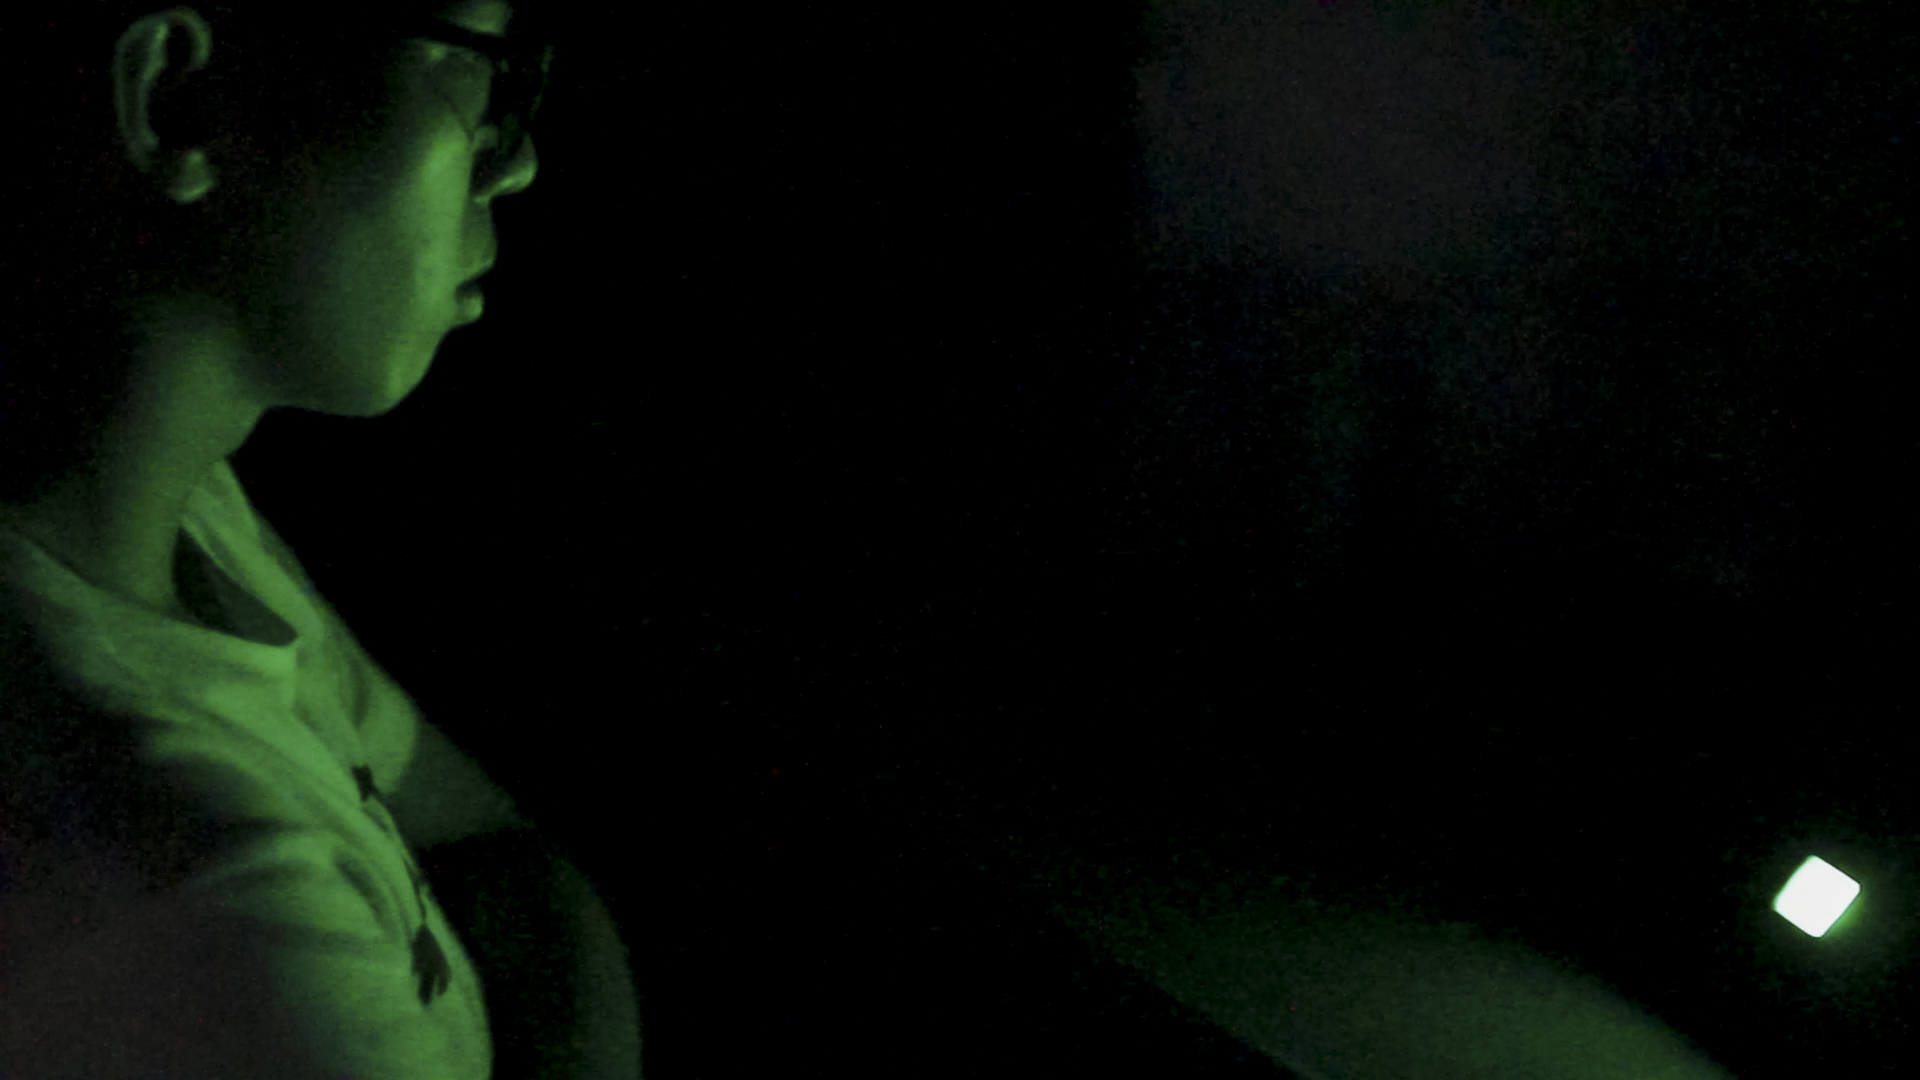
\includegraphics[width=0.8\textwidth]{chapter6/experi.jpg}
	\caption{While in experiment}
\end{figure}

\section{Visual stimulator}


\begin{figure}[ht]
	\centering
	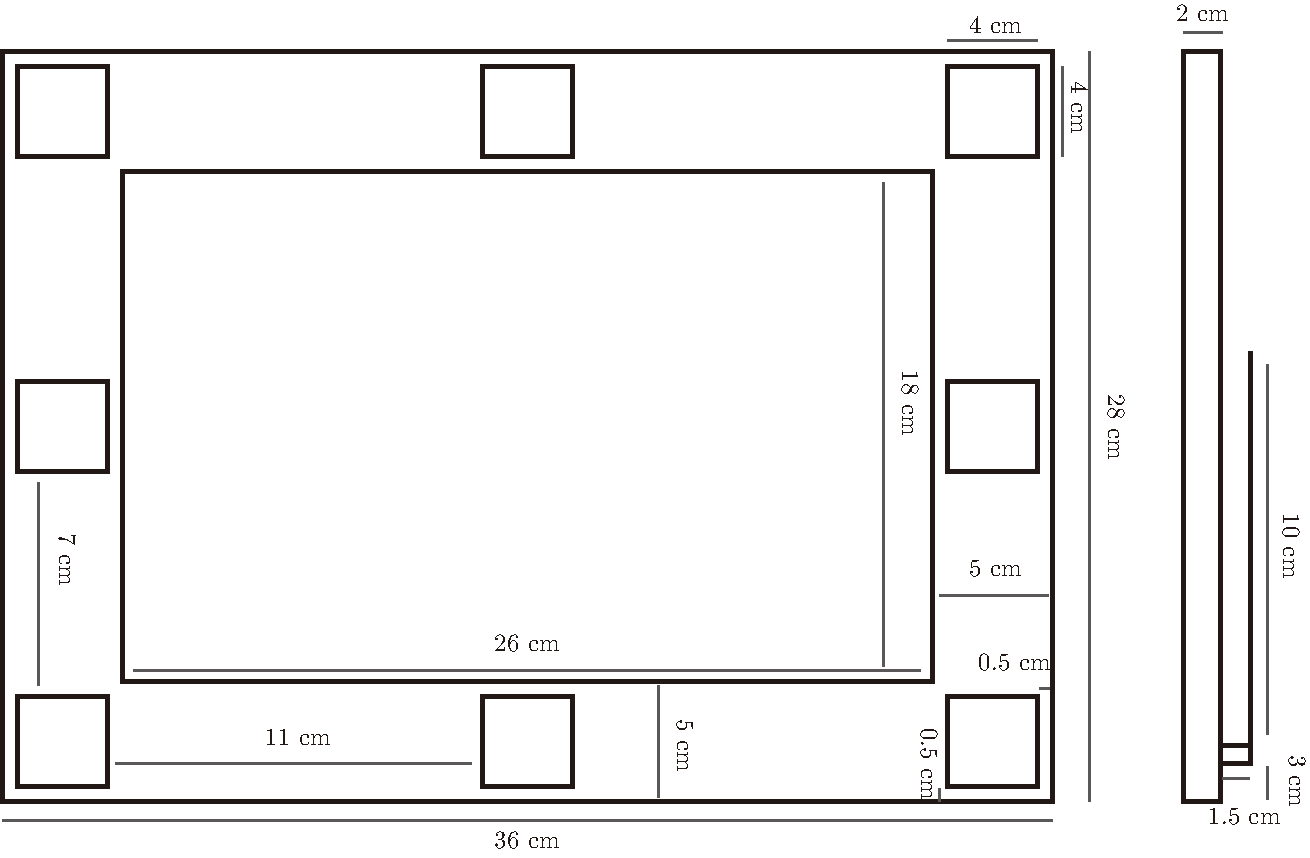
\includegraphics[width=0.8\textwidth]{chapter6/blueprint.pdf}
	\caption{Blueprint of Visual Stimulator}
\end{figure}

\begin{figure}[ht]
	\centering
	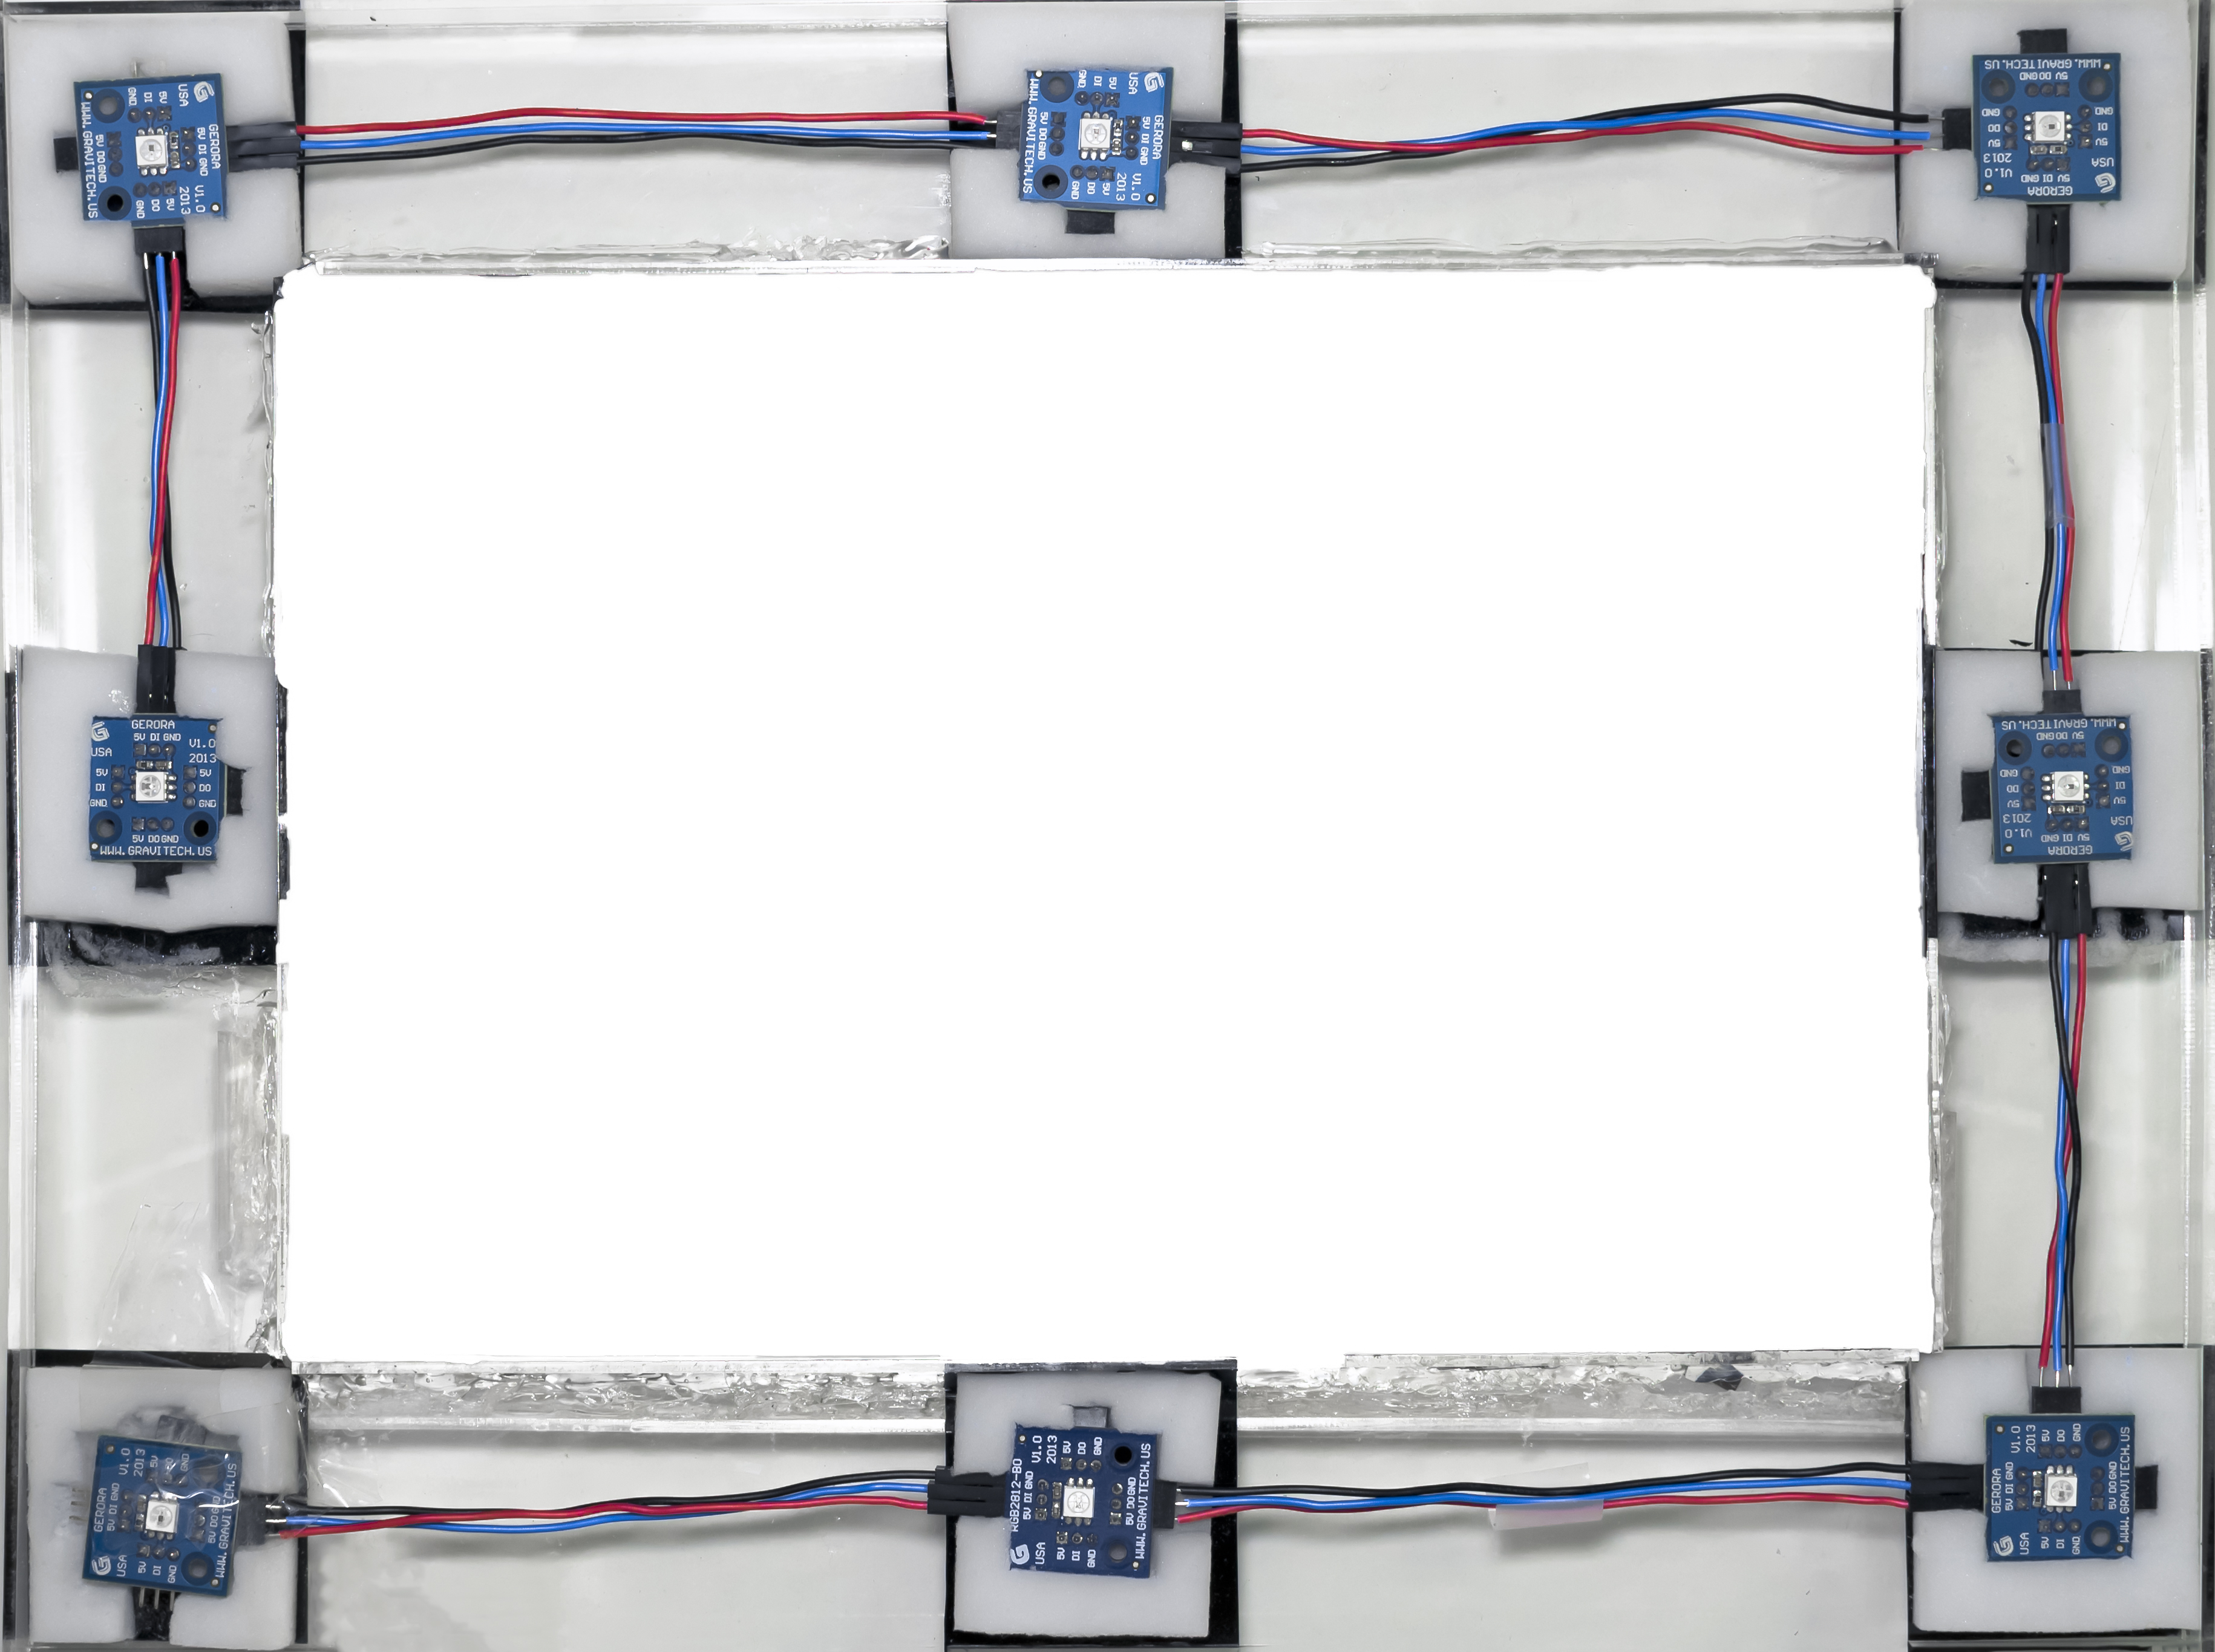
\includegraphics[width=0.8\textwidth]{chapter6/frame_LED.jpg}
	\caption{Visual Stimulator with LEDs wireing}
\end{figure}

\begin{figure}[ht]
	\centering
	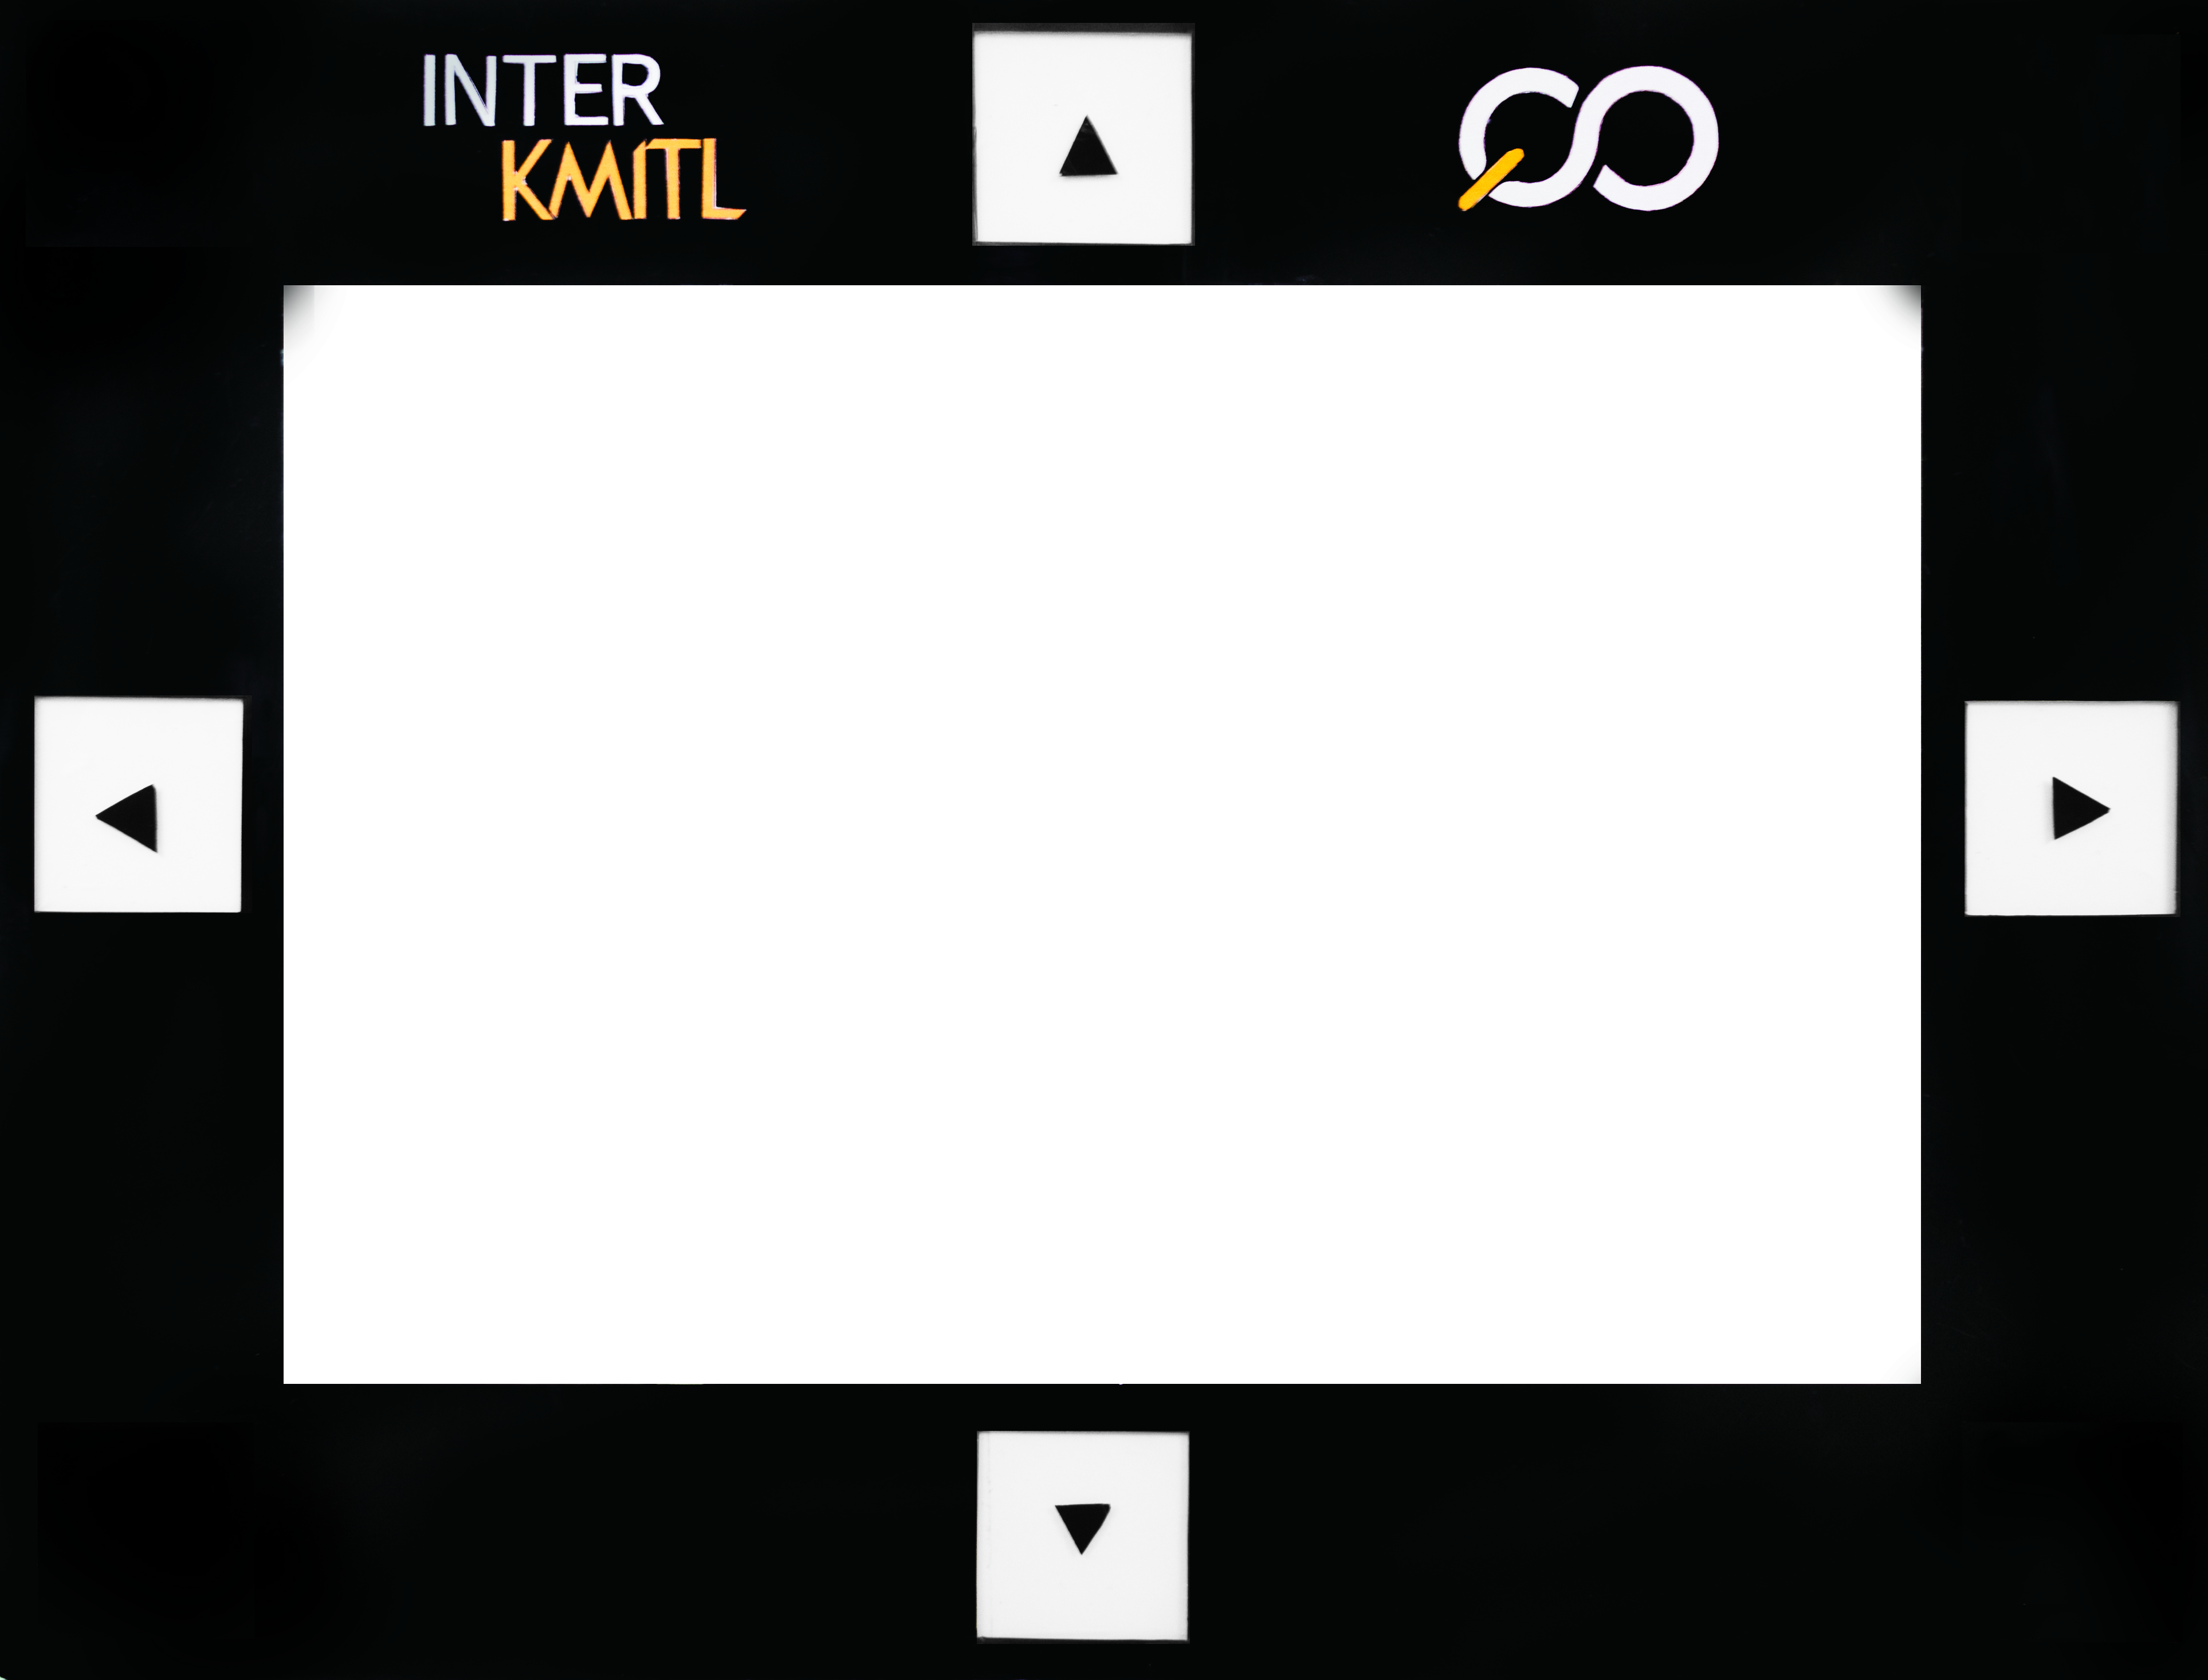
\includegraphics[width=0.8\textwidth]{chapter7/frame_4.jpg}
	\caption{Visual Stimulator with four targets used for ERPs}
\end{figure}

\begin{figure}[ht]
	\centering
	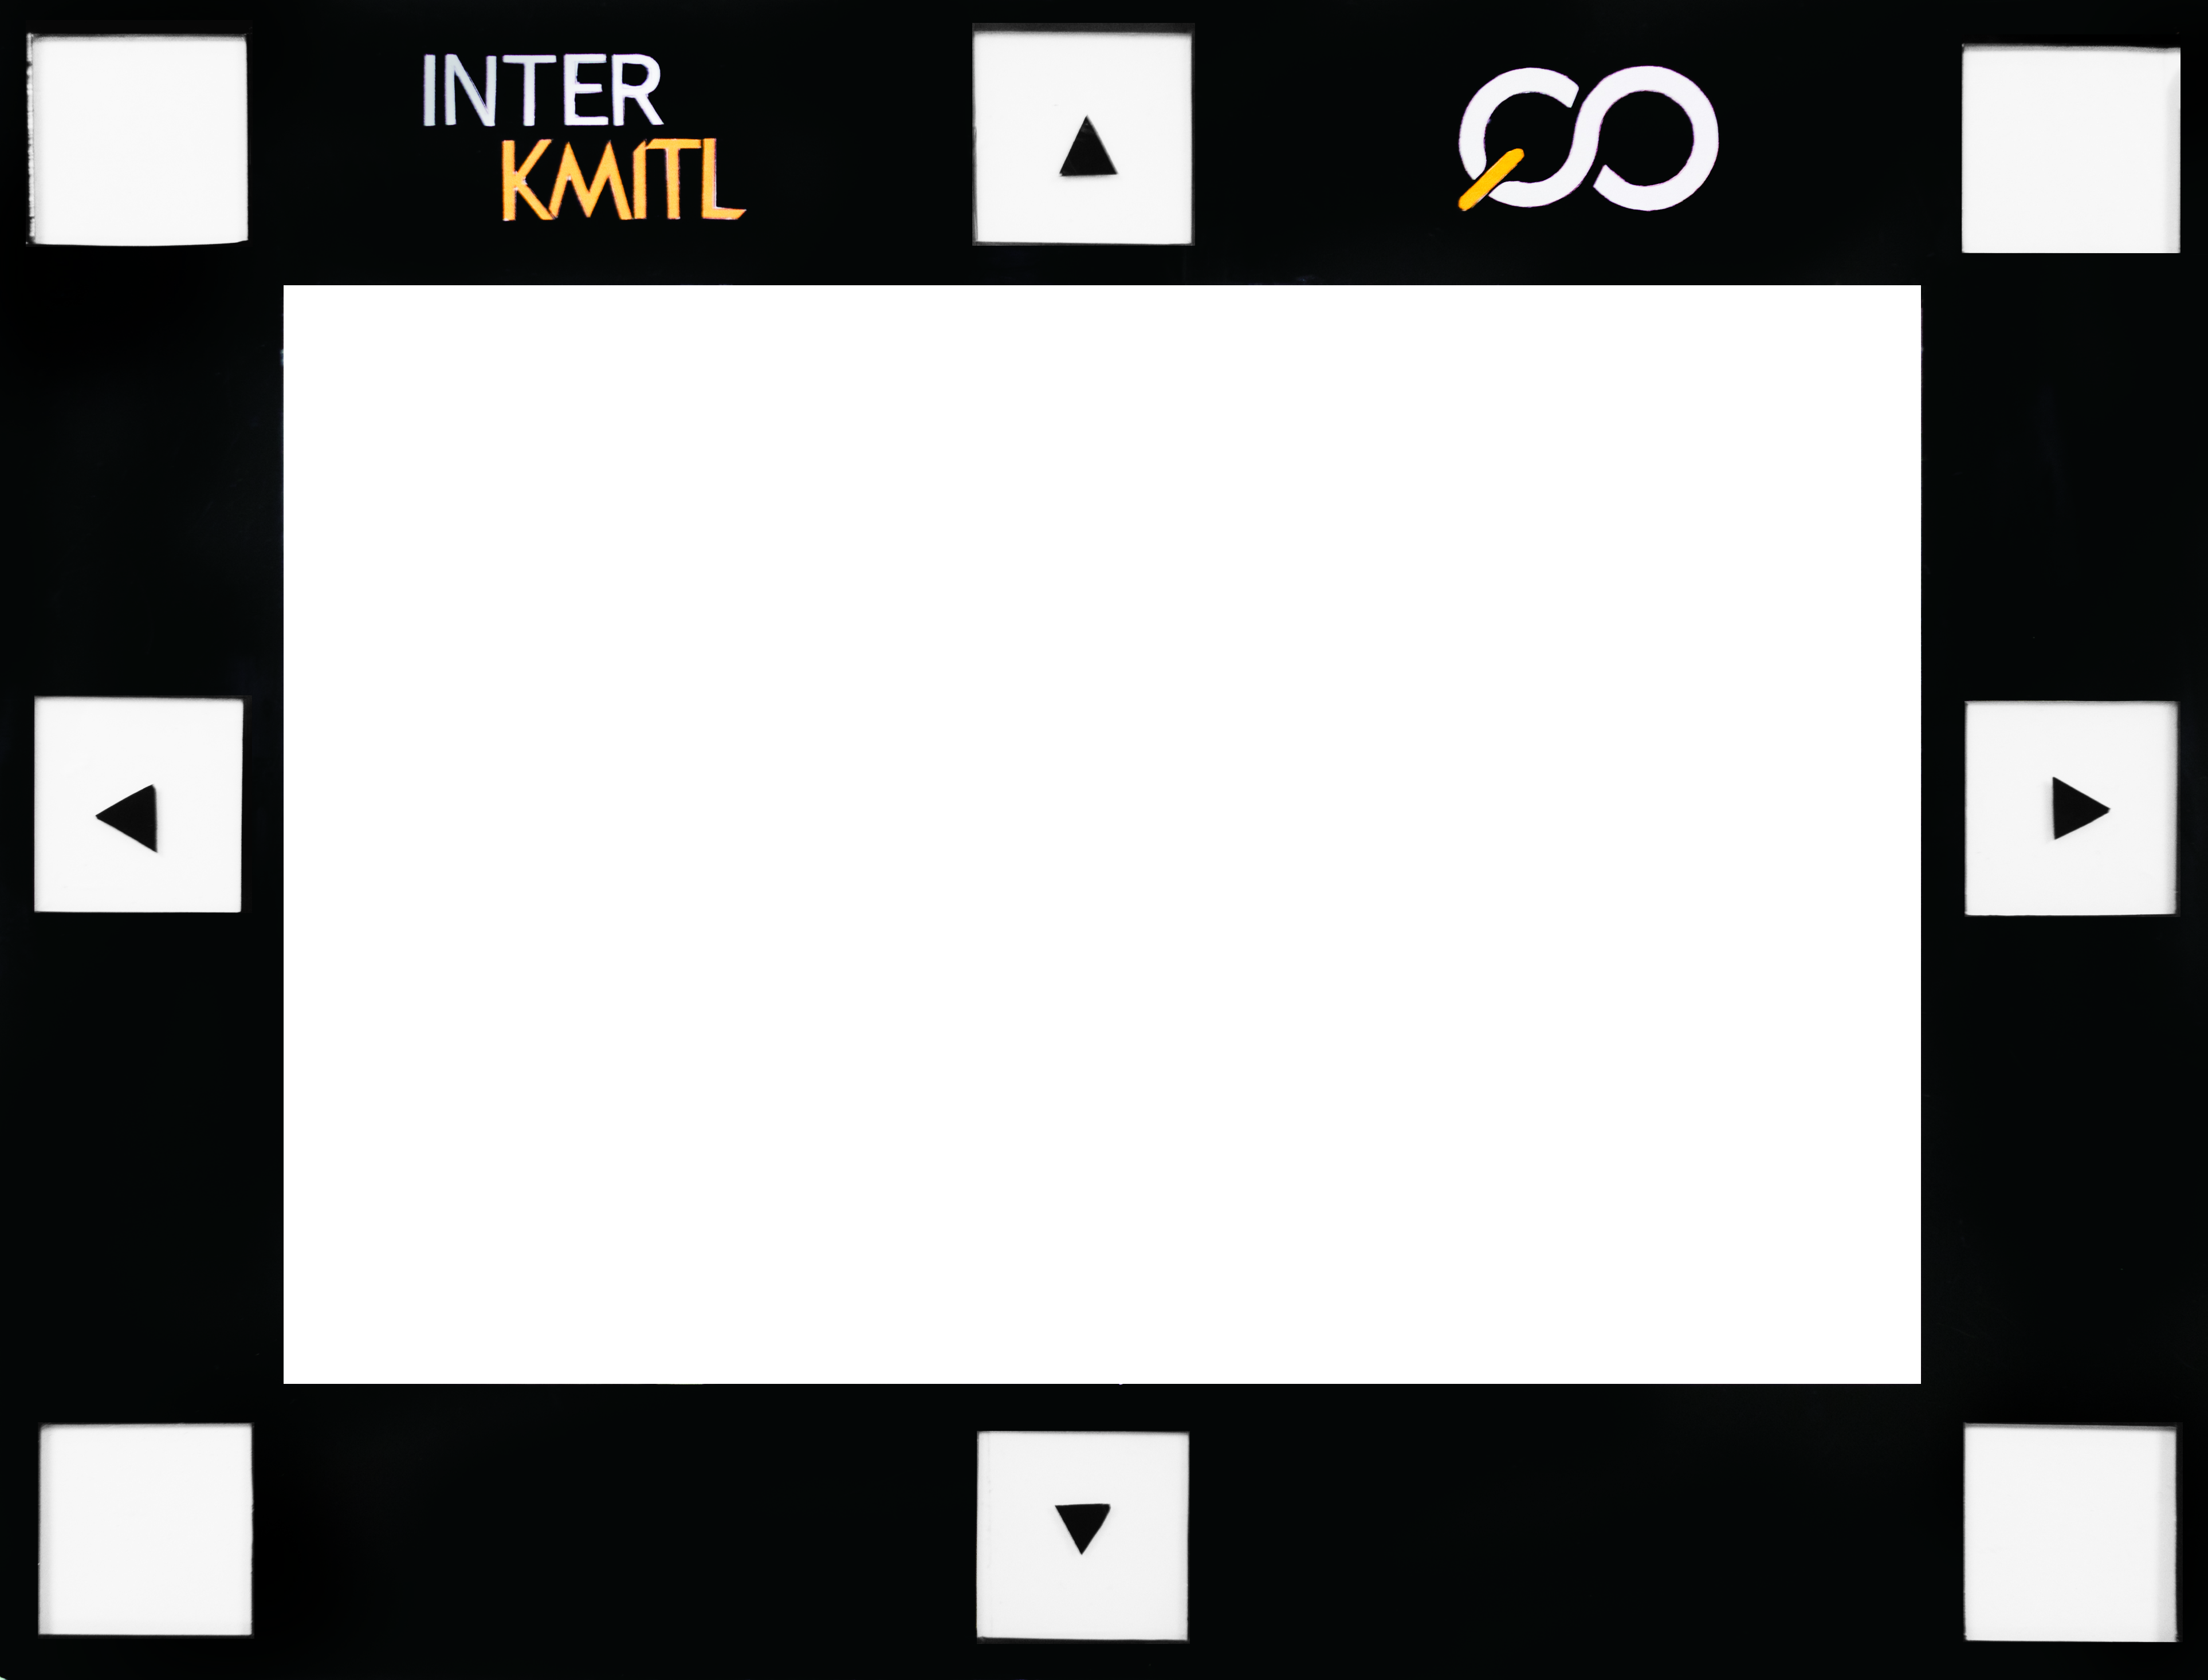
\includegraphics[width=0.5\textwidth]{chapter7/frame_8.jpg}
	\caption{Visual Stimulator with eight targets used for SSVEP}
\end{figure}

\section{Visual stimulator parameter}